\documentclass[12pt]{article}

\usepackage{sbc-template}

\usepackage{graphicx,url}


\usepackage[utf8]{inputenc}  
% UTF-8 encoding is recommended by ShareLaTex
\sloppy

\title{IIT Kharagpur, IARC Team Description Paper}

\address{
Aditya Agarwal, Gaurav Gardi, Kumar Ankit, Kumar Krishna Agarwal, \\
Manash Pratim Das, Sairam K, Soumyadeep Mukherjee, Vishnu Sharma \\ 
\textit{IIT Kharagpur, India}
}

\begin{document}
\maketitle
\begin{abstract}
\\
\begin{center}\textbf{ABSTRACT}\end{center}
This paper reports the current preparation strategy of Aerial Robotics Kharagpur,
participating in IARC Mission 7 2016. Our main goal includes robust, indoor 
localization in GPS denied environments supported by optical flow sensors. 
Other features like ground i-robots detection and differentiation between the 
target bots and patrol bots is also discussed, followed by a brief description 
of the herding algorithm AI algorithm to be used.
\end{abstract}


\section{INTRODUCTION}
Our research group, Aerial Robotics Kharagpur, started in January 2015 with IARC 
being the prime target. Hence we started on with the problem statement of IARC 
mission 7. Our team was organized into two major domains, which are "controls" 
and "software". Keeping Robotics Operating System (ROS) as the base we developed 
our simulation environment in ROS and Gazebo in order to speed up the software 
development and testing while the hardware gets ready. As mission 7 is based 
indoor, hence we made April Tags based indoor true value setup.

\section{SIMULATION}
Gazebo, an open source robotics simulator is used to simulate the robot along with 
the mathematical, physical and visualization model. It also emulates the environment 
with the physics and other interactive robots. We have make ROS plugin for the behaviour 
of i-robots, whereas the quadcopter model,
is made on top of hector\_gazebo, supported by JSBSim, ArduCopter, RotorS, mavros,
ardupilot\_sitl\_gazebo plugin.

\begin{center}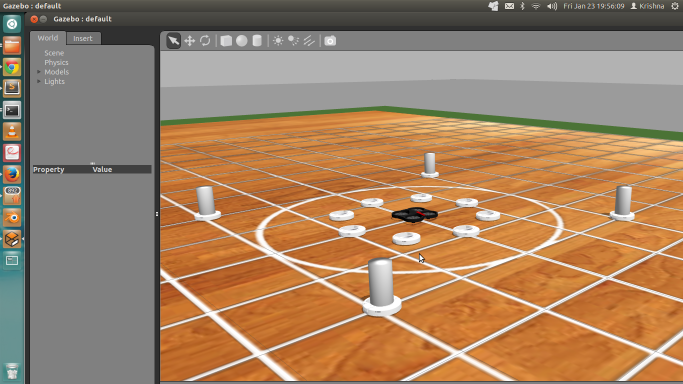
\includegraphics[scale=0.5]{image23} \\
\textbf{Figure 1. Gazebo Simulator.}\end{center}

\section{OVERALL SYSTEM DESIGN}
\begin{center}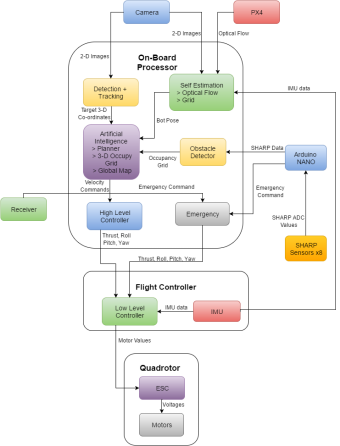
\includegraphics{image22} \\
\textbf{Figure 2. The above is our system design.}\end{center}

\section{LOCALIZATION}
For indoor localization of the quadcopter, we use optical flow and grid localization methods, 
based on px4flow optical flow sensor and bottom camera respectively. The sensor data is fed into, 
an EKF/UKF state estimator that gives the estimated quadcopter pose.

\subsection{Grid Localization}
\subsubsection{Detecting the Grid}
\begin{itemize}
  \item The image is acquired from the on-board cameras on the quadcopter.
  \item The lines in the image are first filtered out and isolated by using segmentation, implemented using the Canny edge detector. 
    \begin{center}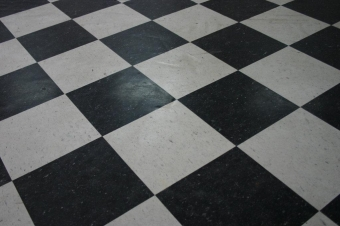
\includegraphics{image25} \\
    \textbf{Figure 3. Image before canny is applied.}\end{center}
    
    \begin{center}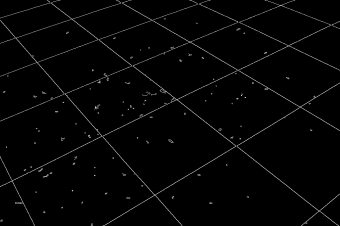
\includegraphics{image24} \\
    \textbf{Figure 4. Image after Canny edge detection is applied.}\end{center}
  \item Once Canny is applied, erosion and dilation is performed on the image to remove noise.
  \item The lines are identified by using a Hough transform on the image.  
  \item After the Hough transform is applied and the lines found, the intersection points of these lines are identified as nodes of the grid.
    \begin{center}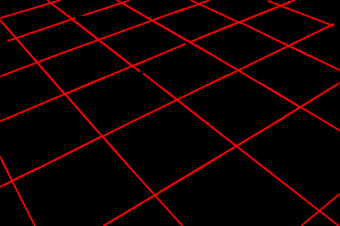
\includegraphics{image27} \\
    \textbf{Figure 5. Image after Hough transform is applied(on Canny filtered image).}\end{center}
\end{itemize}

\subsubsection{Grid Following}
This is achieved by Line following.
\begin{itemize}
    \item The destination node is found.
    \item If the robot is required to proceed from point (x1,y1) to (x2,y2), the robot first finds the nodes that are between these two points.
    \item It then traverses the grid by following the lines connecting these nodes, keeping either x coordinate or y coordinate constant while following each line.
    \item At each node, commands are sent to the robot to turn left, right or to move forward or backward to traverse the lines as described above.
\end{itemize}

\section{GROUND ROBOT DETECTION AND TRACKING}
    \subsection{Detection}
        \subsubsection{Ellipse Detection}
            \begin{itemize}
                \item The detection of each Ground bot will be done with a modified form of Randomized Hough Transform(RHT), fully described in reference, to detect ellipses that correspond to the edges of the bots. 
                \item Two points are selected as the ends of a major axis, and a third point on the assumed ellipse is selected randomly and the vote of the accumulator is done on the length of the minor axis.
            
            \end{itemize}
        \subsubsection{Hog Based SVM Detection}
            \begin{itemize}
                \item Train HOG based classifier by using multiple images of ground robot and then run SVM detector.
            \end{itemize}
        \subsubsection{Template Matching}
            \begin{itemize}
                \item OpenCV Template Matching which is a technique for finding areas of an image that match (are similar) to a template image (patch).
            \end{itemize}
        \subsubsection{YUV Based Segmentation}
         \begin{itemize}
             \item YUV Based Cube Segmentation of Ground Robots followed by blob detection and extraction.
         \end{itemize}
         
    \subsection{Position Estimation}
        Once the bots are detected, the noise associated with the dynamic observables of the moving bot will be filtered out using a Kalman filter to enable tracking of the bot.  This is achieved by the following steps:
        \begin{itemize}
            \item The Kalman filter takes in the measured position of the bot(which in this case is the centre of the ellipse detected by the RHT) as well as its velocity from the video feed.
            \item The position can also be estimated by integrating velocity over time (which incorporates the covariance between the position and velocity). This is called the predicted position.
            \item The error associated with each of these quantities is also found by calculating the expected noise in the readings. The error is estimated as a Gaussian function. 
            \item These two quantities (measured and predicted positions) are compared and the best guess of the bot’s position is made by considering it to be the configuration for which both estimates are most likely after incorporating the associated errors.
        \end{itemize}
    
    \subsection{Tracking of Multiple Robots}
        \begin{itemize}
            \item Having found the most probable position of each bot using the Kalman filter, the next step is to track multiple bots.
            \item A cost matrix is created which incorporates the direction in which the bots had been moving, the distance of the updated estimates of positions from the previous estimates, the expected collisions as well as the expected turns.
            \item The cost matrix is run through the Hungarian algorithm to associate the updated positions with the previous positions, thus giving an identity to each bot, and enabling multiple bot tracking.
        \end{itemize}

\section{OBSTACLE AVOIDANCE}
    IARC consists of moving obstacle robots which need to be avoided when they are on the way of the desired trajectory and path.
    \\ \\
    Obstacles Description: 4 Ground Robots with Cylinders attached on top of them to form vertical moving obstacles.
    \\ \\ 
    \textbf{Avoidance Algorithm Overview:} \\
    The Obstacle Avoidance in IARC does not need to be global as the number of obstacles are less in number. So, we use eight sharp sensors attached on all four arms and between two propellers which measures the distance between the sensor and nearest obstacle. If the obstacle is closer than a threshold then multiple kinds of action can be taken:
    \begin{itemize}
        \item Wait for Obstacle to Move out of Path
        \item Avoid Obstacle by Creating a New Trajectory around the obstacle and come back to desired trajectory.
    \end{itemize}
    \begin{center}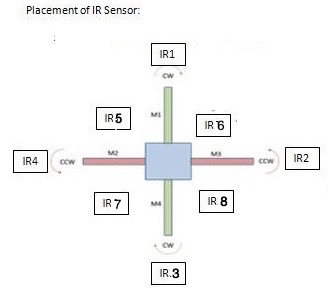
\includegraphics{image26} \\
    \textbf{Figure 6. Placement of IR sensor on the quadcopter.}\end{center}\\

        \subsubsection*{Procedure I:}
            \begin{itemize}
                \item Interrupt Control for IR is triggered as soon as an obstacle comes closer than 40cm from any IR.
                \item Depending on IR from 1-8 and comparing with velocity direction of robot, in case they are same, the robot is halted at the same position or commanded to follow line in reverse till last node is found.
            \end{itemize}}
        \subsubsection*{Procedure II:}
            \begin{itemize}
                \item Trajectory Generation Module is used to generate trajectories from node to node via the lines or directly.
                \item This trajectory generation is recalculated on obstacle trigger and a visible graph is created around the obstacle and followed till next grid node.
            \end{itemize}

\section{SYSTEM CONTROL}
It is advisable for control design to simplify the model in order to comply with the real-time constraints of the embedded control loop. Hence, hub forces and rolling moments are neglected and thrust and drag coefficients are supposed constant. \\
The system can be rewritten in state-space form \(X^{d} = f(X, U)\) with \(U\) inputs vector and \(X\) state vector chosen as follows:
\[ X = [ \phi \quad \dot{\phi} \quad \theta \quad \dot{\theta} \quad \psi \quad \dot{\psi} \quad z \quad \dot{z} \quad x \quad \dot{x} \quad y \quad \dot{y}]^{T} \]

Inputs Vector:
\[ U = [U_1 \quad U_2 \quad U_3 \quad U_4] \]

where the inputs are mapped by:
\[U_1 = b(\Omega_1^2 + \Omega_2^2 + \Omega_3^2 + \Omega_4^2) \]
\[U_2 = b(-\Omega_2^2 + \Omega_4^2)\]
\[U_3 = b(\Omega_1^2 - \Omega_3^2)\]
\[U_4 = d(-\Omega_1^2 + \Omega_2^2 - \Omega_3^2 + \Omega_4^2)\]

\begin{center}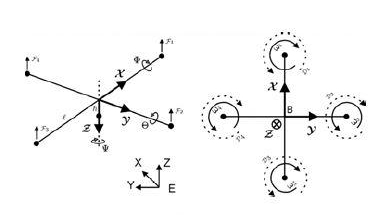
\includegraphics{image30} \\
\textbf{Figure 7. Co-ordinate system.}\end{center}\\

\[f(X, U) = \left[ \begin{array}{c}
                                    \dot{\phi} \\ 
                                    \dot{\theta}\dot{\psi}a_1 + \dot{\theta}a_2\Omega_r + b_1U_2 \\
                                    \dot{\theta} \\
                                    \dot{\phi}\dot{\psi}a_3 - \dot{\psi}a_4\Omega_r + b_2U_3 \\
                                    \dot{\psi} \\
                                    \dot{\theta}\dot{\phi}a_5 + b_3U_4 \\
                                    \dot{z} \\
                                    g - (cos\phi cos\theta)\frac{1}{m} U_1 \\
                                    \dot{x} \\
                                    u_x\frac{1}{m} U_1 \\
                                    \dot{y} \\
                                    u_y\frac{1}{m} U_1
            \end{array} \right] \]

\[ a_1 = (I_y_y - I_z_z)/I_x_x\]
\[ a_2 = J_r/I_x_X\]
\[ a_3 = (I_z_z - I_x_x)/I_y_Y \]
\[ a_4 = J_r/I_y_y \]
\[ a_5 = (I_x_x - I_y_y)/I_z_z \]
\[ b_1 = l/I_x_x \]
\[ b_2 = l/I_y_y \]
\[ b_3 = 1/I_z_z \]
\\
\[ u_x = cos\varphi sin\theta cos\Psi + sin\varphi sin\psi \]
\[ u_y = cos\varphi sin\theta cos\Psi - sin\varphi sin\psi \]

\[\left[ \begin{array}{c} p \\ q \\ r \end{array} \right] = \begin{bmatrix} c\theta & 0 & -c\phi s\theta \\ 0 & 1 & s\phi \\ s\theta & 0 & c\phi c\theta \end{bmatrix} \times \left[ \begin{array}{c} \dot{\phi} \\ \dot{\theta} \\ \dot{\psi} \end{array} \right]\] \\

\subsubsection*{Angular velocity components in quadcopter frame}
\[ r_T(t) = \left[\begin{array}{c} x(t) \\ y(t) \\ z(t) \\ \psi(t)  \end{array} \right] \]
\[ e_p = r_T(t) - r \]
\[ e_v = \dot{r}_T(t) - \dot{r}

Let \(r = [x \quad y \quad z]^{T}\) and \( (\ddot{r}_T(t) - \ddot{r}_c) + k_{d,x}e_v + k_{p,x}e_p = 0 \)

We want: $\ddot{r_c}$ : Commanded acceleration, calculated by controller.

We have,
\begin{center}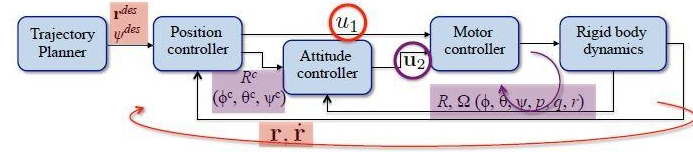
\includegraphics[scale=0.5]{image38} \\
\textbf{Figure 8. Control loop.}\end{center}\\

\[ m \ddot{r} = \left[\begin{array}{c} 0 \\ 0 \\ -mg \end{array} \right] + R\left[\begin{array}{0} 0 \\ 0 \\ F_1 + F_2 + F_3 + F_4 \end{array} \right]\]

\[ I\left[\begin{array}{0} \dot{p} \\ \dot{q} \\ \dot{r} \end{array}\right] = \left[\begin{array}{0} L(F_2 - F_4) \\ L(F_3 - F_1) \\ M_1 - M_2 + M_3 - M_4 \end{array}\right] - \left[\begin{array}{0} p \\ q \\ r \end{array}\right] \times I\left[\begin{array}{0} p \\ q \\ r \end{array}\right]
\]

\subsubsection*{Control for Hovering:}
Linearized dynamics at the hover configuration
\[ (u_1 \sim mg, \theta \sim 0, \phi \sim 0, \psi \sim \psi_0) \]
\[ u_2 \sim 0, p \sim 0, q \sim 0, r \sim 0 \]
\\

Hence,
\[ I\left[\begin{array}{0} \dot{p} \\ \dot{q} \\ \dot{r} \end{array}\right] = \left[\begin{array}{0} L(F_2 - F_4) \\ L(F_3 - F_1) \\ M_1 - M_2 + M_3 - M_4 \end{array}\right]
\]

\[ u_2 = \left[\begin{array}{c} k_{p,\phi}(\phi_c - \phi) + k_{d, \phi}(p_c - p) \\ k_{p,\theta}(\theta_c - \theta) + k_{d, \theta}(q_c - q) \\ k_{p,\psi}(\psi_c - \psi) + k_{d, \psi}(r_c - r)\end{array} \right] \]

\section{IARC ROBOT: ALBATROSS DESCRIPTION}
\begin{center}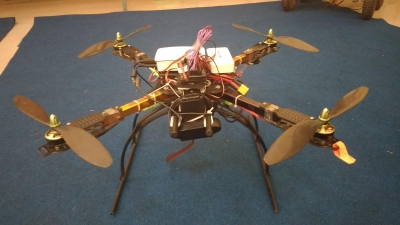
\includegraphics{image41} \\
\textbf{Figure 9. Quadcopter: Albatross.}\end{center}\\
\subsection{Configuration}
\begin{itemize}
    \item Odroid XU4 : High Level Controller
    \item APM : Low Level Controller
    \item ESC     : Electronic Speed Controller, 45A OPTO
    \item LiPo     : 11.1V, 3s, 5000mAh, 20C
    \item Motors: 850kv BLDC
    \item Propellers : 11” x 4.7”
    \item Camera : 30fps, Field of View - 78 degrees, Aspect Ratio - 16:9
    \item Receiver : 6 channel PPM
    \item Frame : Glass Fibre X frame
\end{itemize}

\section{HERDING ALGORITHM AI}
\subsection{Greedy Method}
\begin{itemize}
    \item The motif of this algorithm is to stop the ground bots from crossing a line while shifting the line ahead if the area behind is cleared of the bots.
    \item Before takeoff, the quadcopter will be fed with the direction information about the green and red lines. The direction information will tell where is the red line (east/west/north/south).
    \item Once the quadcopter takes off, it will hold altitude at 1.5m (from ground) and hold position on the nearest node while holding its yaw.
    \item As it knows the general direction of the red line, so it turns on the node to a heading that is aligned with a grid line along the general direction of the red line.
    \item It then follows the grid to:
        \begin{itemize}
            \item Detect the position of red line. Let us call it L0
            \item Track back to the line ahead of it. L1.
            \item Move to the end of L1. L(present) = L1.
        \end{itemize}
    \item The quadcopter will now start making  “search & clear” maneuver. This maneuver is a loop that involves:
        \begin{itemize}
        \item Moving along line L(present) to search for ground bots.
        \item If ground bots are found, then it will mark the location and predict trajectory of each one of them. 
        \item Once the search is complete it will target the ground bots it encountered and make strategic landing for each one of them to turn them in the general direction of the green line. This process will clear the particular section it can view while moving along the line and will ensure section present in L < L(present)
        \item Once the section is clear it will go to an end of L(present) ++. And continue the loop.
        \end{itemize}
    \item So we keep clearing the area and pushing the ground bots until they cross the green line.
\end{itemize}
\begin{center}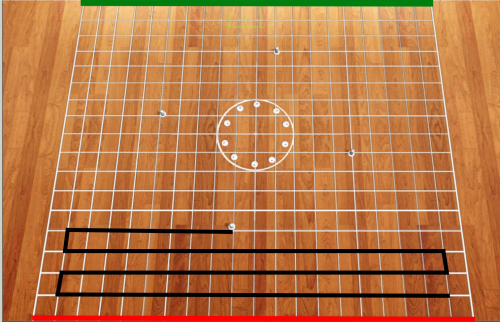
\includegraphics[scale=0.7]{image28} \\
\textbf{Figure 10. Herding algorithm visualization.}\end{center}\\
Assumption: Our robot is faster than the ground robots.

\section{EMERGENCY KILL SWITCH}
We have three level of control on the quadcopter: Wifi-software, standard Radio Control link and "IARC Common Kill Switch"[17] as given in IARC website.
As required in the competition, we have a hardware independent safety mechanism to act as a kill switch in case of an emergency that will cut power
to the electronic speed controllers. RC control link can be used for manual override control of the quadcopter or to change ArduCopter mode to LAND, while the same can be achieved by mavros commands over Wifi link to the on-board computer. 

\section{TRUE VALUE SETUP}
Setup of a ground truth system is essential to register ground truth data. Obtained data can be used to evaluate, test and benchmark algorithms related to localization, mapping and motion planning in quadcopters. This setup should be robust to illumination changes, shadows and arena modifications. Such setup would even help in many different strategies to work upon further, like tracking of system, game strategies and for easy debugging. \\ \\
Depth perception from conventional stereo vision is based on the triangulation principle as mentioned. [1, 2, 6, 8, 9]. The 3D position of quadcopter can be obtained by the intersection of the two rays passing through the camera optical centers and its 2D projections in each image, but object disparity is an important cue for position estimation. We use two cameras arranged on a baseline, such that their view fields overlap at the desired object distance. By taking a picture with each camera, we capture the scene from two different viewpoints. Hence, a correspondence needs to be established between two images regions that correspond to some physical feature in space. Then the depth can be reconstructed using triangulation, which is discussed further. \\
We use April Tags[16] placed on the quadcopter to track it.
\begin{center}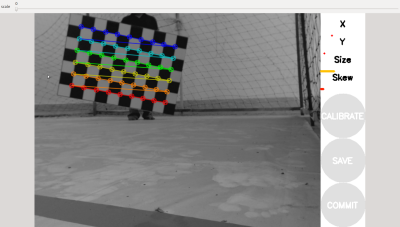
\includegraphics{image42} \\
\textbf{Figure 11. Left and right Camera Calibration using 9*6 checkerboard}\end{center}\\

\section{References}
\begin{enumerate}
    \item Aerodynamics for Engineering Students by E. L. Houghton, P.W.Carpenter, Butterworth-Heinemann Publication.
    \item Fundamentals of Aerodynamics by John David Anderson, McGraw-Hill Publication.
    \item Engineer's Aerodynamics by S. M. Yahya, John wiley & sons publication. 
    \item P. Pounds, R. Mahony, and P. Corke, “Modelling and Control of a Large Quadrotor Robot,” in Control Engineering Practice, vol. 18, pp. 691 – 699, 2010. 
    \item \href{http://ieeexplore.ieee.org/iel5/5076472/5152175/05152390.pdf?arnumber=5152390}{P. Pounds and R. Mahony, “Design principles of large quadrotors for practical applications,” in Proceedings of the IEEE International Conference on Robotics and Automation (ICRA), pp. 3265 –3270, May 2009.}
    \item R. S. Samir Bouabdallah, Pierpaolo Murrieri Autonomous Robots, vol. 18, Mar 2005.
    \item J. Irizarry, M. Gheisari and B. Walker, “Usability assessment of drone technology as safety inspection tools” in Journal of Information Technology in Construction, Sept 2012. 
    \item T. Iwai, A. Nunnikhoven, E. Rodger, E. Roggatz, P. Rose and J. Warning, “Quadcopter with collective and cyclic control” in Iowa State University, Project Design, Fall 2010. 
    \item Honig, Z. (2011) “T-Hawk UAV enters Fukushima danger zone, returns with video.” 6:48PM April 21, 2011, retrieved on April 22, 2011. 
    \item \href{http://9to5mac.com/2011/06/15/awesome-use-of-an-ipad-and-the-parrot-ar-drone/}{Zibreg. C. (2011) “Awesome use of an iPad and the Parrot AR Drone.”} 
    \item Faigl, J., Krajnik, T., Vonasek, V., and Preucil, L. (2010) “Surveillance planning with localization uncertainty for mobile robots.” 3rd Israeli Conference on Robotic. 
    \item Ng, W.S., and Sharlin, E. (2011) “Collocated interaction with flying robots.” Technical Report 2011-998-10, Department of Computer Science, University of Calgary, Calgary, Canada (2011). 
    \item Higuchi, K., Shimada, T., and Rekimoto, J. (2011) “Flying sports assistant: external visual imagery representation for sports training.” 2nd Augmented Human International Conference, New York, NY, USA, ACM 7:1–7:4.
    \item \href{http://www.aviationsystemsdivision.arc.nasa.gov/publications/hitl/rtsim/Toms.pdf}{T. S. Alderete, “Simulator aero model implementation.” NASA Ames Research Center, Moffett Field, California.}
    \item H. Bouadi and M. Tadjine, “Nonlinear observer design and sliding mode control of four rotors helicopter,” Proceedings of World Academy of Science, Engineering and Technology, vol. 25, pp. 225–230, 2007.
    \item \href{https://april.eecs.umich.edu/papers/details.php?name=olson2010tags}{Edwin Olson, "AprilTag: A robust and flexible multi-purpose fiducial system"}
    \item \href{http://www.aerialroboticscompetition.org/downloads/killswitch.zip}{The IARC common safety switch}
\end{enumerate}
\end{document}
